\section{4点関数}

この節では強結合領域$\beta J \gg 1$における4点関数を論じる。
disorder-averageを取る事によって最も一般的な4点関数は
\begin{align}
	\average{\psi_i(t_1)\psi_i(t_2)\psi_j(t_3)\psi_j(t_4)}
\end{align}
という形に制限される。
これを$i$と$j$について平均を取ったものを考える:
\begin{align}
	\frac{1}{N^2}\sum_{i,j=1}^{N}\average{T\psi_i(t_1)\psi_i(t_2)\psi_j(t_3)\psi_j(t_4)}
	= G(t_{12})G(t_{34}) + \frac{1}{N}\mathcal{F}(t_1, \cdots, t_4).
	\label{eq:fourpointfunc}
\end{align}
以下では$\mathcal{F}$について解析する。

\begin{figure}[h]
	\centering
	\vspace{1cm}
	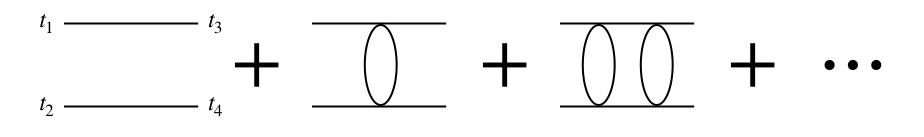
\includegraphics[width=13cm]{figures/ladderDiagram}
	\caption{\eqref{eq:fourpointfunc}式の$1/N$の項を表すダイアグラム。
		特に$q=4$の場合について描画した。ラダーダイアグラムと呼ぶ。}
	\label{fig:ladderdiagram}
\end{figure}

$\mathcal{F}$を表すダイアグラムはラダーダイアグラムである(図\ref{fig:ladderdiagram})。
$n$個の輪があるものを$\mathcal{F}_n$とすると、計算するべきは
\begin{align}
	\mathcal{F} = \sum_n \mathcal{F}_n
\end{align}
である。
図\ref{fig:ladderdiagram}の最初にある輪を持たないラダーダイアグラムは単なるプロパゲーターの積である:
\begin{align}
	\mathcal{F}_0(t_1, \cdots, t_4) = -G(t_{13})G(t_{24}) + G(t_{14})G(t_{23}).
\end{align}
次に並ぶ、輪を1個だけ持つラダーダイアグラムでは、輪の端の位置について積分した形で与えられる:
\begin{align}
	\mathcal{F}_1(t_1, &\cdots, t_4)\nonumber\\
	&= J^2(q - 1)\int dtdt'\ \left(
		G(t_1 - t)G(t_2 - t')G(t - t')^{q-2}G(t - t_3)G(t' - t_4) - (t_3 \leftrightarrow t_4)
	\right).
\end{align}
積分の前にある$q-1$という因子は、どの線をレールや輪にするかのパターン数に起因する。
上述した2つのラダーダイアグラム$\mathcal{F}_0$、$\mathcal{F}_1$に限らず、
全てのラダーダイアグラムは$1/N$に比例する。

あるラダーダイアグラム$\mathcal{F}_n$と次の$\mathcal{F}_{n+1}$の間には
\begin{align}
	\mathcal{F}_{n+1}(t_1, \cdots, t_4)
	= \int dtdt'\ K(t_1, t_2; t, t')\mathcal{F}_n(t, t', t_3, t_4)
	\label{eq:F_n+1_and_F_n}
\end{align}
という漸化式的な関係がある。
ここで積分核$K$は
\begin{align}
	K(t_1, t_2; t_3, t_4) = -J^2(q-1)G(t_{13})G(t_{24})G(t_{34})^{q-2}
	\label{eq:def_of_K}
\end{align}
である。
\eqref{eq:F_n+1_and_F_n}式の計算では、$K$の最初の2つの変数を1つめの添字、残りの2つを2つ目の添字
と見なす事によって積分を行列計算としてしまうのが便利である(行列$K$は2変数反対称関数の空間に作用する)。
こうする事で全てのラダーダイアグラムの総和を
\begin{align}
	\mathcal{F}
	= \sum_{n=0}^{\infty}\mathcal{F}_n
	= \sum_{n=0}^{\infty}K^n \mathcal{F}_0
	= \frac{1}{1 - K}\mathcal{F}_0
	\label{eq:geometric_series_of_F}
\end{align}
という様に表す事ができる。
これを更に計算するために、以下では$K$を対角化する事を考える。
\eqref{eq:def_of_K}式による定義では$K$は対称行列ではないが、
次のような操作により対称化する事が可能である:
\begin{align}
	\tilde{K}(t_1, t_2; t_3, t_4) \equiv
	|G(t_{12})|^{\frac{q-2}{2}}K(t_1, t_2; t_3, t_4)|G(t_{34})|^{\frac{2-q}{2}}.
\end{align}
従って$K$は固有関数(固有ベクトル)の完全系を持つとして良い。
今、固有値を$g(\alpha)$、固有関数を$v_{\alpha}(t_a, t_b)$とすると
\begin{align}
	\int dt_a dt_b\ v_{\alpha}(t_a, t_b)K(t_a, t_b; t_3, t_4)
	= g(\alpha)v_{\alpha}(t_3, t_4),
\end{align}
あるいは行列とベクトルの様に表記するなら
\begin{align}
	Kv_{\alpha} = g(\alpha)v_{\alpha}
\end{align}
である。
固有関数$v_{\alpha}$を用いて\eqref{eq:geometric_series_of_F}式の行列$\frac{1}{1-K}$
を展開すると
\begin{align}
	\mathcal{F}
	= \sum_{\alpha} v_{\alpha}\frac{1}{1 - g(\alpha)}\langle v_{\alpha}, \mathcal{F}_0\rangle
\end{align}
と書ける。
ここで$\langle v_{\alpha}, \mathcal{F}_0\rangle$は何らかの内積を表わす。
$\mathcal{F}_0$は$v_{\alpha}$を用いれば
\begin{align}
	\mathcal{F}_0(t_1, t_2, t_3, t_4)
	= \sum_{\alpha} \gamma_{0\alpha}(t_1, t_2)v_{\alpha}(t_3, t_4)
\end{align}
と展開でき、これを使うと$\langle v_{\alpha}, \mathcal{F}_0\rangle = \gamma_{0\alpha}$より
\begin{align}
	\mathcal{F}
	= \sum_{\alpha} v_{\alpha}\frac{\gamma_{0\alpha}}{1 - g(\alpha)}
\end{align}
となる。

\subsection{Kの対角化}
ここまでの話は一般の$\beta J$について成り立つ。
解析を進めるために、以下では共変対称性の成り立つ極限$\beta J \gg 1$で考える。
よって2点関数は$\eqref{eq:conformal_ansatz}$式の$G_c(t)$で与えられる。
\eqref{eq:conformal_ansatz}式を\eqref{eq:def_of_K}式に代入すると、
$K$の共変不変なものとして
\begin{align}
	K_c(t_1, t_2; t_3, t_4)
	= -\frac{1}{\alpha_0}
		\frac{\sgn(t_{13})\sgn(t_{24})}{|t_{13}|^{2\Delta}|t_{24}|^{2\Delta}|t_{34}|^{2-4\Delta}}
	\label{eq:confomarl_K}
\end{align}
を得る。ここで
\begin{align}
	\alpha_0 \equiv \frac{2\pi q}{(q-1)(q-2)\tan\frac{\pi}{q}}
\end{align}
である。
$K_c$を対角化した暁には、実は固有関数の中に固有値$g(\alpha) = 1$を持つものも存在する。
従って\eqref{eq:geometric_series_of_F}式の級数は発散するが、これは共変極限から摂動的に少し
ずれる事によって対処する事ができる。
それを議論するまでは、ひとまず\eqref{eq:confomarl_K}式を用いる事にする。

$K_c$の対角化では共変不変性を活用する事になる。
SYK模型は時間1次元しか持たないので、1次元共形場理論$\mathrm{CFT}_1$であり
\footnote{1次元の場の量子論は本質的に量子力学なので、
Conformal Quantum Mechanicsの頭文字を取ってCQMと表記する事もある。}、
共変変換群は$SL(2, \mathbb{R})$で与えられる\cite{andrzejewski}:
\begin{align}
	L_p = t_1^p\partial_1 + t_2^p\partial_2,\hspace{20pt}
	[L_p, L_q] = (q - p)L_{p + q - 1},\hspace{30pt}
	p,q = 0, 1, 2.
\end{align}
ここから$\tilde{L}_p = |t_{12}|^{-3/2}L_p|t_{12}|^{3/2}$とすると便利とかあるけど
この3/2って多分$q=4$の時のなので、$K$を対称化する式と可換であることを用いて一般の$q$について
やってみるしかない。

\pagebreak
